% ---
% Capa
% ---
\imprimircapa
% ---

% ---
% Folha de rosto
% (o * indica que haverá a ficha bibliográfica)
% ---
\imprimirfolhaderosto*
% ---

% ---
% Inserir a ficha bibliografica
% ---
% http://ficha.bu.ufsc.br/
\begin{fichacatalografica}
	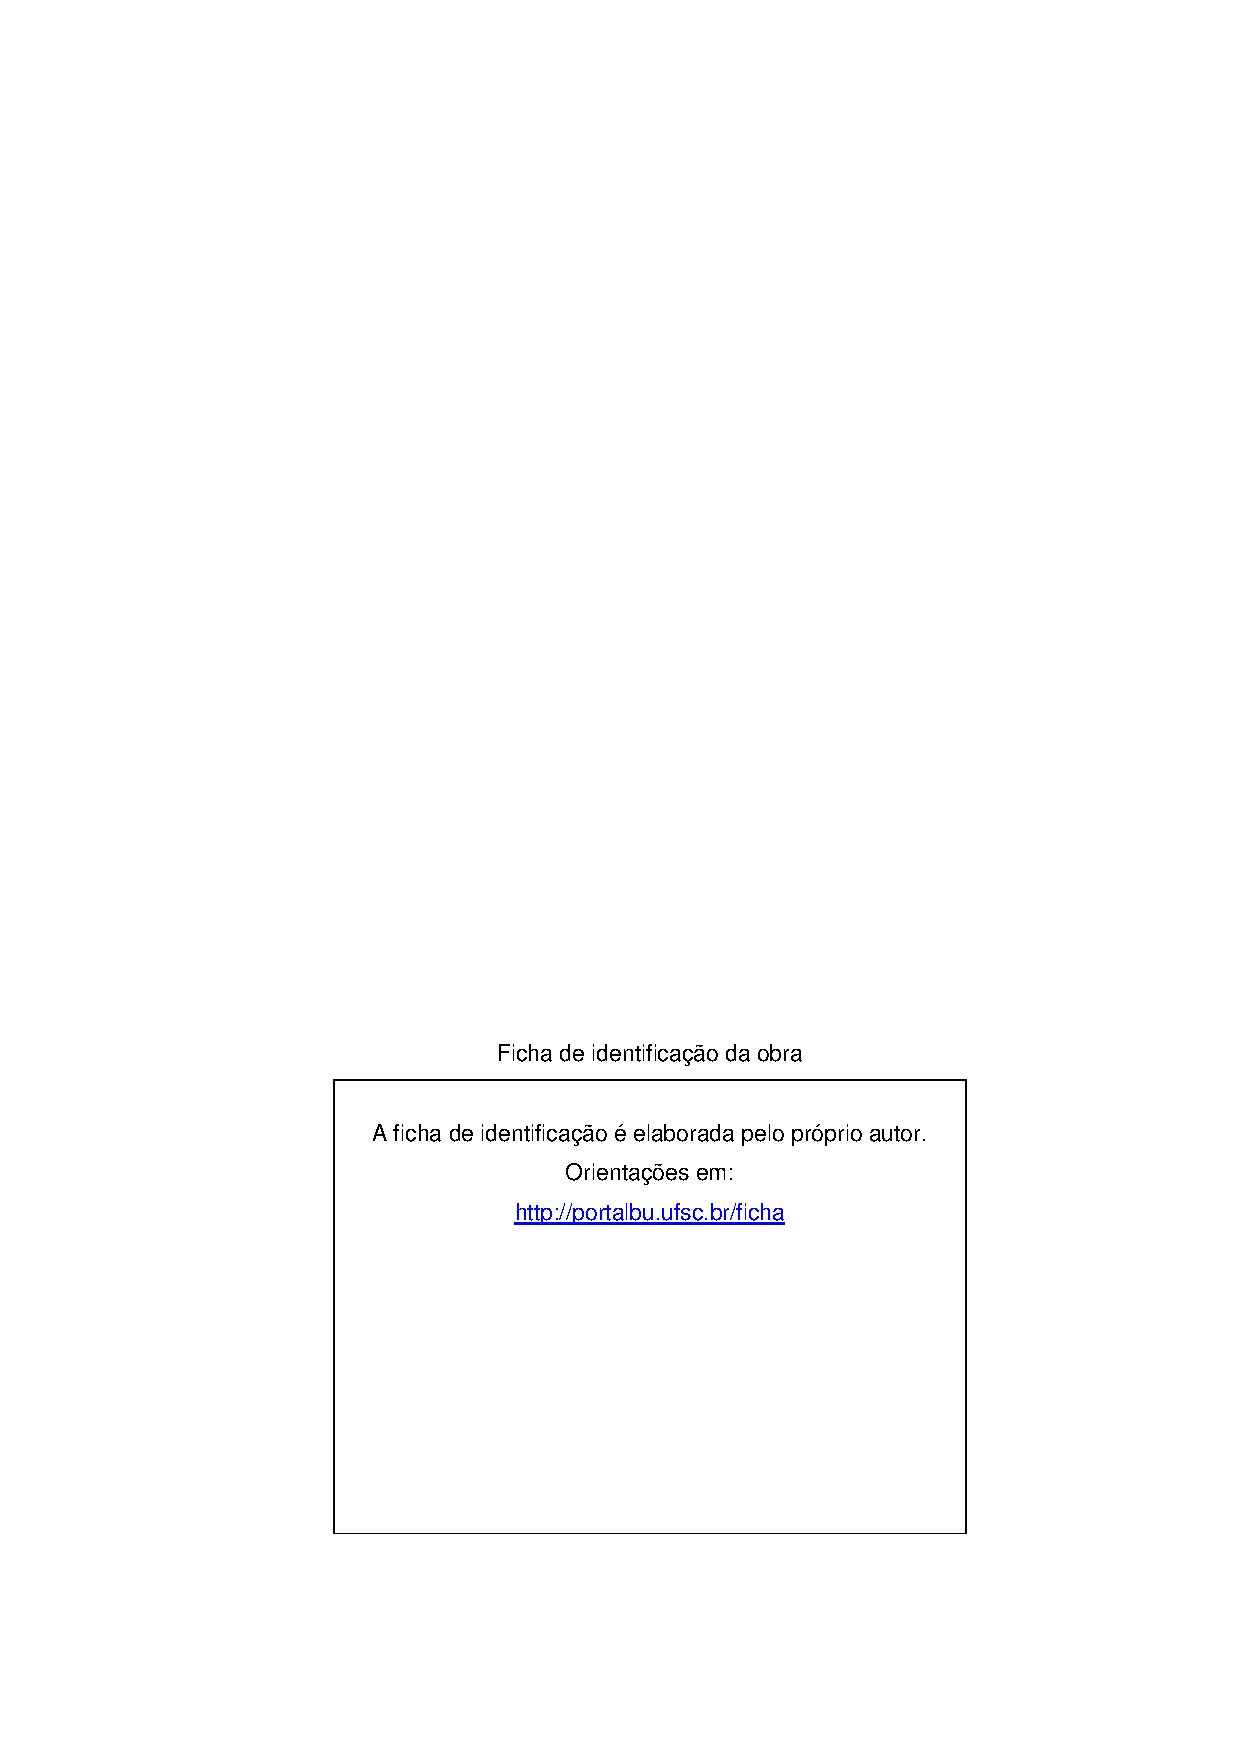
\includepdf{beforetext/Ficha_Catalografica.pdf}
\end{fichacatalografica}
% ---

% ---
% Inserir folha de aprovação
% ---
\begin{folhadeaprovacao}
	\OnehalfSpacing
	\centering
	\imprimirautor\\%
	\vspace*{10pt}		
	\textbf{\imprimirtitulo}%
	\ifnotempty{\imprimirsubtitulo}{:~\imprimirsubtitulo}\\%
	%		\vspace*{31.5pt}%3\baselineskip
	\vspace*{\baselineskip}
	
	This dissertation was evaluated in the context of the subject DAS5511 (Course Final Project) and approved in its final form by the \imprimircurso\\
	%Esta monografia foi julgada no contexto da disciplina DAS5511 (Projeto de Fim de Curso) e aprovada em sua forma final pelo \imprimircurso\\
	\vspace*{\baselineskip}
	Florianópolis, July 2nd, 2022.\\
	
	%%%%%%%%%%%%%%%%%%%%%%%%%%%%%%%%%%%%%%%%%%%%%
	%IMPORTANT: no signatures are required below!
	%%%%%%%%%%%%%%%%%%%%%%%%%%%%%%%%%%%%%%%%%%%%%
	
	\vspace*{2\baselineskip}
	%\rule{0.4\textwidth}{0.4pt}\\
	Prof. Hector Bessa Silveira, Dr.\\
	Course Coordinator\\
	
	\vspace*{\baselineskip}
	\textbf{Examining Board:} \\
	
	
	\vspace*{2\baselineskip}
	%\rule{0.4\textwidth}{0.4pt}\\
	Prof. Eduardo Camponogara, Dr.\\
	Advisor and Supervisor \\
	UFSC/CTC/DAS\\
	
	\vspace*{2\baselineskip}
	%\rule{0.4\textwidth}{0.4pt}\\
	Prof. Danilo Silva, Dr.\\
	Evaluator \\
	UFSC/CTC/EEL\\
	
	\vspace*{2\baselineskip}
	%\rule{0.4\textwidth}{0.4pt}\\
	Prof. Marcelo de Lellis Costa de Oliveira, Dr.\\
	Board President \\
	UFSC/CTC/DAS
\end{folhadeaprovacao}
% ---

% ---
% Dedicatória
% ---
\begin{dedicatoria}
	\vspace*{\fill}
	\noindent
	\begin{adjustwidth*}{}{5.5cm} 
		\raggedleft       
		This work is dedicated to my father.
	\end{adjustwidth*}
\end{dedicatoria}
% ---

% ---
% Agradecimentos
% ---
\begin{agradecimentos}
    First and foremost, this work was made possible thanks to the guidance of Prof. Eduardo Camponogara, who accompanied me from the very beginning.
    Also thanks to my father and my girlfriend, who supported me in many different ways.
    Finally, I would like to thank all the masters who inspired me and helped me develop the faculties necessary for this work, specially Prof. João Goulart, Prof. Ivan Pontual, Prof. Gustavo Donatelli, Prof. Eduardo Camponogara (again), Jonathan Krauß, and Prof. Danilo Silva.
\end{agradecimentos}
% ---

% ---
% Epígrafe
% ---
\begin{epigrafe}
	\vspace*{\fill}
	\begin{flushright}
		\textit{``The sciences do not try to explain, they hardly even try to interpret, they mainly make models. By a model is meant a mathematical construct which, with the addition of certain verbal interpretations, describes observed phenomena. The justification of such a mathematical construct is solely and precisely that it is expected to work - that is correctly to describe phenomena from a reasonably wide area. Furthermore, it must satisfy certain esthetic criteria - that is, in relation to how much it describes, it must be rather simple.''\\
		\emph{John von Neumann} apud \emph{\textcite{leary_unity_1955}}}
	\end{flushright}
\end{epigrafe}
% ---

% ---
% RESUMOS
% ---

% resumo em português
\setlength{\absparsep}{18pt} % ajusta o espaçamento dos parágrafos do resumo
\begin{resumo}
	\SingleSpacing
	\Glspl{PINN} and \glspl{DEQ} are novel approaches that approximate deep learning's representational power to applications with realistic requirements such as robustness, data scarcity and explainability.
	\Glspl{PINN} propose an efficient way to train neural networks to model physical phenomena.
	\Glspl{DEQ} are a new model architecture that can provide more representational power with fewer parameters.
	This work aims to study both and apply them to solve \glspl{IVP} of \glspl{ODE}, in an approach coined \gls{PIDEQ}.
	We implement the proposed approach and test it, analyzing the impacts of the multiple hyperparameters in the approximate solution of the  Van der Pol oscillator.
	Our results show that indeed \gls{PIDEQ} models are able to solve \glspl{IVP}, providing approximate solutions with small errors.
% 	\textbf{Instruções do padrão genérico de TCCs da BU:}
	% No resumo são ressaltados o objetivo da pesquisa, o método utilizado, as discussões e os resultados com destaque apenas para os pontos principais. O resumo deve ser significativo, composto de uma sequência de frases concisas, afirmativas, e não de uma enumeração de tópicos. Não deve conter citações. Deve usar o verbo na voz ativa e na terceira pessoa do singular. O texto do resumo deve ser digitado, em um único bloco, sem espaço de parágrafo. O espaçamento entre linhas é simples e o tamanho da fonte é 12. Abaixo do resumo, informar as palavras-chave (palavras ou expressões significativas retiradas do texto) ou, termos retirados de thesaurus da área. Deve conter de 150 a 500 palavras. O resumo é elaborado de acordo com a NBR 6028. \textbf{Instruções da Coordenação do PFC:} o resumo deve contextualizar o trabalho e descrever de forma sucinta o problema, a solução proposta, a metodologia utilizada e os resultados obtidos. Tudo de forma bem resumida e direta, sem entrar em detalhes técnicos.
	
	\textbf{Keywords}: Physics-Informed Neural Network; Deep Equilibrium Model; Implict Model; Initial-Value Problem; Deep Learning.
\end{resumo}

% resumo em inglês
\begin{resumo}[Resumo]
	\SingleSpacing
	\begin{otherlanguage*}{brazil}
	    Redes neurais para solução de problemas físicos, denominadas \emph{physics-informed neural networks} (PINNs), e modelos profundos de equilíbrio (do inglês, DEQs), são contribuições recentes que facilitam o uso de modelos de aprendizagem profunda, conhecidos pela capacidade representativa, de aplicações com requisitos realistas de robustez, explicabilidade e escassez de dados.
	    PINNs se mostraram uma forma eficiente de treinar redes neurais para modelar fenômenos físicos.
	    DEQs, por outro lado, empregam uma nova arquitetura que promete mais capacidade de representação com menos parâmetros.
	    Este trabalho consiste em um estudo de ambos, além de uma aplicação que combina-os para resolver problemas de valor inicial de equações diferenciais ordinárias, com um modelo chamado PIDEQ.
	    A abordagem proposta para resolver esse tipo de problema foi implementada e testada utilizando o oscilador de Van der Pol, com uma análise de impacto dos seus diferentes hiperparâmetros.
	    Os resultados mostram que, de fato, é possível treinar um PIDEQ para resolver o problema proposto, gerando soluções aproximadas com baixo erro.
		

	   % \textbf{Palavras-chave}: Palavra-chave 1. Palavra-chave 2. Palavra-chave 3.
	\end{otherlanguage*}
\end{resumo}

%% resumo em francês 
%\begin{resumo}[Résumé]
% \begin{otherlanguage*}{french}
%    Il s'agit d'un résumé en français.
% 
%   \textbf{Mots-clés}: latex. abntex. publication de textes.
% \end{otherlanguage*}
%\end{resumo}
%
%% resumo em espanhol
%\begin{resumo}[Resumen]
% \begin{otherlanguage*}{spanish}
%   Este es el resumen en español.
%  
%   \textbf{Palabras clave}: latex. abntex. publicación de textos.
% \end{otherlanguage*}
%\end{resumo}
%% ---

{%hidelinks
	\hypersetup{hidelinks}
	% ---
	% inserir lista de ilustrações
	% ---
	\pdfbookmark[0]{\listfigurename}{lof}
	\listoffigures*
	\cleardoublepage
	% ---
	
	% ---
	% inserir lista de quadros
	% ---
% 	\pdfbookmark[0]{\listofquadrosname}{loq}
% 	\listofquadros*
% 	\cleardoublepage
	% ---
	
	% ---
	% inserir lista de tabelas
	% ---
	\pdfbookmark[0]{\listtablename}{lot}
	\listoftables*
	\cleardoublepage
	% ---
	
	% ---
	% inserir lista de abreviaturas e siglas (devem ser declarados no preambulo)
	% ---
	\imprimirlistadesiglas
	% ---
	
	% ---
	% inserir lista de símbolos (devem ser declarados no preambulo)
	% ---
	\imprimirlistadesimbolos
	% ---
	
	% ---
	% inserir o sumario
	% ---
	\pdfbookmark[0]{\contentsname}{toc}
	\tableofcontents*
	\cleardoublepage
	
}%hidelinks
% ---
